% - open-world, why it's hard
%  + closed-world guarantees data seen during testing is same as during training, this is unrealistic
%  + open-world is more realistic and significantly more challenging, how to classify similar or overlapping data?
%  + composed of several areas of ML investigation, e.g. CL and class discovery, but major area of investigation is identifying when exactly something new has been encountered
%As machine learning (ML) continues to develop and pervade modern technology, it has increasingly encountered circumstances in which methods are applied to real-world settings. Inevitably, proposed ML models are transitioned from the curated laboratory environments of research to the clinical environments of industry, medicine, public service, and other such applications \cite{sarker2021machine,nozari2024ai,bertolini2021machine,deo2015machine,mohseni2021practical}. This presents a major challenge for ML as most ML models to date have relied on a significant limiting assumption: that data encountered by models during testing (i.e. in application) is \emph{drawn from the same distribution} as data used by the model for training. This assumption is commonly known as the \textbf{closed-world} assumption, referring to the notion that the model learns from -- and is used in -- a ``closed-world'' of the same distribution of data \cite{bendale2016towards,fei2016breaking,joseph2021towards,scheirer2012toward,he2015delving,krizhevsky2012imagenet}. In laboratory settings, this assumption is a convenient tool for developing ML methods, allowing for greater efficiency and reproducibility. However, the real world almost never follows the closed-world assumption. Instead, data in realistic settings commonly originates from sources (i.e. distributions) \emph{not seen during training} (intuitively denoted as the \textbf{open-world} setting) \cite{joseph2021towards,scheirer2012toward,drummond2006open}. ML models applied in open-world settings thus encounter testing data instances that were not encountered during training, originating from different distributions. This is a critical problem because ML models must be designed to handle the unknown data present in real-world settings, but it is impossible to prepare for this data during training due to the infinite amount of unknown classes and the intractable nature of learning the entire true space of the input data \cite{joseph2021towards,scheirer2012toward,zhou2001small}.
Modern technology has rapidly embraced machine learning (ML) as a component in myriad tools, products, services, etc. The development and pervasiveness of ML has exposed it to real-world settings and the associated circumstances involved with application in realistic environments. ML models, as they are transitioned from research environments protected by curated laboratory settings, are expected to operate effectively and reliably in clinical environments of industry, medicine, public service, and other such areas \cite{sarker2021machine,nozari2024ai,bertolini2021machine,deo2015machine,mohseni2021practical}. However, this transition embodies a major problem for ML. Many ML models, methods, and techniques rely on a significant limiting assumption: data encountered during testing (i.e. in real-world settings and applications) is \textit{drawn from the same distribution} as data encountered during training. This \textbf{closed-world} assumption entails that any given ML system learns from, and is used in, a ``closed-world'' of data, where all encountered samples are drawn from the same distribution.

The real-world rarely follows the closed-world assumption. Application settings frequently contain data that originates from distributions (i.e. data sources) that have \textit{not been seen during training}. That is, encountered data during testing may originate from a data distribution different from that encountered during training. This setting is referred to as the \textbf{open-world} setting \cite{joseph2021towards,scheirer2012toward,drummond2006open}. ML systems previously designed under the closed-world assumption cannot be directly applied in open-world settings, as there is no longer any guarantee that encountered testing data is from the same distribution as prepared for during training. Furthermore, an obstacle exists in the development of new systems and techniques for open-world settings. Open-world ML systems must prepare to handle the unknown data present in real-world application settings, but it is impossible to anticipate what data distribution(s) will be encountered once deployed. Training on all possible data is intractable, as it is impossible to consider the entire space of input data and expose ML models to all possible data distributions during training. In fact, existing research details that attempting to train models to understand all possible data is fruitless, as there are an infinite number of unknown classes and models cannot feasibly learn knowledge of the entire set of possible data \cite{joseph2021towards,scheirer2012toward}. Even attempting to model the space of data outside the training data distribution is unrealistic as an impossibly large amount of data would be required to properly represent the true data distribution \cite{zhou2001small}. This presents a critical problem for ML.

%  + open-world is more realistic and significantly more challenging, how to classify similar or overlapping data?
The open-world problem for ML contains several tasks that revolve around handling the existence of unseen data distributions instead of attempting to learn them. One primary task focuses on the ability of ML systems to distinguish when encountered test data is from the training data distribution or not \cite{yang2024generalized,sehwag2019analyzing}. This is a broad and intricately complex task space. For example, an ML model is applied on a wildlife observation camera at a nature preserve. The model was previously trained to identify different species of mammals but the scientists are also interested in noting any potential new species in the area. The ML model may encounter some clear deviations from its seen-data distribution encountered during training, e.g. a bird hops across the camera. Birds have many visual features that distinguish them from mammals, including wings, small legs, feathers, and other morphological and visual differences. However, the ML model may encounter other inputs that are less clear. Perhaps the model was trained to recognize coyotes in the preserve but it captures images of a wolf. Coyotes and wolves are not only both mammals but belong to the same genus, sharing many visual features, including four legs, similar body shape, fur, etc. Preparing ML models to handle such subtle deviations in data distribution between training and testing is critical for application in real-world scenarios. This need becomes more potent when considering that there are various sub-species of coyote that may look very similar, or perhaps have never been encountered before. ML models cannot feasibly be prepared to handle these circumstances via training and yet must be able to identify when test data is arbitrarily similar to (or even overlapping with) training data.

%\textcolor{red}{TODO: find a way to add this or elaborate on it, may need to dig up more refs for it though}
%\textcolor{blue}{ALTERNATIVE: This is a critical problem because ML models must be designed to handle the unknown data in real-world settings, but it is impossible to prepare for this data during training due to the infinite amount of unknown classes and intractable nature of learning the entire true set of data \cite{scheirer2012toward,joseph2021towards,zhou2001small}.} This is a serious issue because, as researchers, it is intractable to expose ML models to all possible data distribution during training and yet it is ideal to design models that can handle unknown situations when applied to real problems \textcolor{blue}{citation needed or re-word - Joseph discusses ``infinite'' unknown classes, Scheirer talks about ``cannot have knowledge of entire set'', Zhou ``limited number of negative examples cannot represent the true distribution well''}.

%(critical component of open-world ml is ood detection - simple definition can go here)

%  + composed of several areas of ML investigation, e.g. CL and class discovery, but major area of investigation is identifying when exactly something new has been encountered
% - (sec) OOD detection as key solution component for open-world
%  + exactly the task of identifying when encountered data is NOT from the seen data dist
\section{Out-of-Distribution Detection is Critical for Open-World Application}

%A significant component in addressing the closed-world assumption is imbuing ML models with the ability to detect when data is encountered that has not previously been seen during training. More specifically, an ML model with greater capability to operate in open-world settings must be able to 1) operate as expected when presented with test data from distributions it has seen during training (such data is henceforth referred to as \emph{in-distribution} (ID) data), and 2) detect when presented test data is from a distribution that was not seen during training (\emph{out-of-distribution} data). This problem is referred to as \textbf{Out-of-Distribution} (OoD) \textbf{Detection}, in which an ML model must learn how to detect OoD data samples while only being exposed to (i.e. only learning from) ID data samples \cite{hendrycks2017baseline,yang2021generalized}. An ML model that has solved the OoD detection problem can better operate in open-world settings as it can \emph{identify}, during application, when encountered samples are different from samples the model was trained with. This provides such models with greater capabilities to more flexibly respond to unknown situations, a property much desired in engineering and industrial applications \cite{siau2018building,hendrycks2022x,hendrycks2021unsolved,amodei2016concrete,nitsch2021out}.
Preparing ML systems for open-world application encapsulates a large family of artificial intelligence (AI) and ML research directions, ranging from continual learning (CL) to autonomous class discovery to many others. However, the significant underlying component in developing ML for open-world settings is the aforementioned ability to detect when data is encountered that has not previously been seen during training. Specifically, any open-world ML system must be able to leverage the data distribution it has seen, henceforth referred to as the \textit{\gls{id}} data distribution, to detect when presented test data is from a different data distribution, henceforth referred to as the \textit{\gls{ood}} data distribution. This problem is known as \textbf{\gls{ood} Detection}. In \gls{ood} detection, an ML system must distinguish \gls{ood} data samples from \gls{id} data samples during testing after only being exposed to (e.g. only learning from) \gls{id} training data \cite{hendrycks2017baseline,yang2021generalized,cui2022out,lu2025out}. Solving the \gls{ood} detection problem enables ML systems to effectively operate in open-world settings as they can \textit{identify} when encountered samples are different from the samples the model is prepared to handle. This provides significantly more flexibility and capability in real-world ML solutions, enabling them to operate in unknown situations, a property much desired in engineering and industrial applications \cite{siau2018building,hendrycks2022x,hendrycks2021unsolved,amodei2016concrete,nitsch2021out}. \gls{ood} detection is also a fundamental component in other open-world solution methods, such as CL and autonomous class discovery \cite{kim2022theoretical,de2021continual}. The development of \gls{ood} detection is thus essential to the expansion of ML to the domain of open-world settings.

%(existing applications, an example or two here would be ideal (maybe even a figure showing the significance)

%\textcolor{blue}{TODO - figure showing importance of OoD, use car and car with person in front, similar formatting to Nitsch paper (Out-of-Distributino Detection for Automotive Perception)}
\begin{figure}
 \centering
 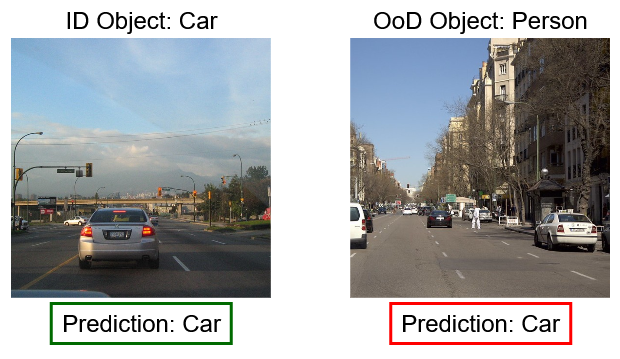
\includegraphics[width=0.9\linewidth]{figures/importance_example_1}

  \caption{OOD detection is a critical ML component necessary in many applications. Inability to identify unknown or unfamiliar data during use could lead to disastrous consequences. It is not enough for ML models to learn ID data, they must be designed with awareness of OOD data.
  }
  \label{fig:intro-ood_importance}
\end{figure}

%In practice, OoD detection has been recognized as a critically important component in myriad applications. In autonomous driving, several studies have studied using OoD detection for more accurate vehicle detection in images and identifying sources of road sign misclassification \cite{nitsch2021out,eykholt2018robust,geiger2012we,muhammad2020deep}. An example of the potential importance of OoD detection in autonomous driving is presented in Figure \ref{fig:intro-ood_importance}. With OoD detection, an ML model could identify the sudden OoD sample (right image) and, for example, activate a failsafe maneuver in order to avoid a catastrophic accident. In robotics, important uses of OoD detection include detecting sensor anomalies and environment-based behavior adaptation \cite{falcini2017deep,farid2022task}. In these cases, OoD detection can be used as a filter for noisy or malformed sensor readings to improve control of robots or prevent inappropriate actions in critical application environments. Benefits have also been noted in the related field of industrial automation, with one particular noteworthy study demonstrating use of OoD detection for identifying damaged products \cite{bergmann2019mvtec}. Studies in medical diagnosis have also identified beneficial applications of OoD detection via identification of abnormal growths, lesions, etc. as well as improving intelligibilty for patient transparency and trust \cite{caruana2015intelligible,schlegl2019f}. Further examples of OoD detection applications can be found in relevant works \cite{yang2021generalized,farid2022task,filos2020can,zhang2021out}.
\gls{ood} detection has already been tested in real-world applications, exhibiting critical importance across myriad settings. One application area with tangible effects is autonomous driving. Studies have investigated the use of \gls{ood} detection for vehicle detection in images and explaining sources of road sign classification mistakes \cite{nitsch2021out,eykholt2018robust,geiger2012we,muhammad2020deep}. An example of the importance of \gls{ood} detection in autonomous driving is illustrated in \ref{fig:intro-ood_importance}. \gls{ood} detection allows ML models to identify sudden \gls{ood} samples (right image), enabling intelligent responses to such situations, e.g. engaging failsafe maneuvers to avoid a catastrophic accident. Another application for \gls{ood} detection is robotics. \gls{ood} detection can be used to detect sensor anomalies or induce environment-based adaptations in robot behavior \cite{falcini2017deep,farid2022task}. In such applications, \gls{ood} detection acts as a filter for noisy sensor readings and improves robot control while preventing inappropriate actions in high-risk or resource-limited task environments. Other applications include industrial automation, where \gls{ood} detection has been evaluated for identification of damaged products \cite{bergmann2019mvtec}. In medical diagnosis, \gls{ood} detection has proven effective at detecting medical anomalies such as abnormal growths, lesions, etc. Additionally, applications improving the intelligibility of medical results for improved patient transparency and trust have leveraged \gls{ood} detection \cite{caruana2015intelligible,schlegl2019f}. More examples of \gls{ood} detection in real-world applications can be found in relevant surveys and research works \cite{yang2021generalized,farid2022task,filos2020can,zhang2021out}.

%\begin{abstract}
%Although out-of-distribution (OOD) detection has been extensively studied, it continues to face challenges in handling OOD data semantically similar to In-Distribution (ID) data. Part of the difficulty arises from the model's inability to learn superior ID class discriminative features. We propose to improve this by segmenting input images into \textit{foreground} and \textit{background} views and combining them with the original input image (original view) in a multi-view learning approach. We present a novel method, called \textbf{\sys}~(\textbf{C}ross-view \textbf{A}ttention of \textbf{S}egmented views for \textbf{O}OD \textbf{D}etection), that learns better discriminative information from all three views and subsequently, fuses them through a novel stacked cross-view attention mechanism to produce the final predictive feature representation. A feature-based OOD method is then applied to the final fused feature for OOD detection, giving major improvements over a range of strong baselines on various near- and far-OOD datasets.
%\sys achieves state-of-the-art performance in various experimental settings with challenging ID and OOD datasets. The \sys \textbf{codebase} is submitted in the supplementary materials.
%\end{abstract}
%
%Machine learning (ML) models have been largely built and deployed under the \textit{closed-world} assumption \citep{joseph2021towards}, where the test data distribution is assumed to be the same as the training data distribution. However, this assumption is often violated in real-world scenarios, as a deployed model may encounter test instances of classes not seen during training. To reliably operate in such \textit{open-world} settings \citep{liu2023ai}, ML models should not only recognize instances of known (or seen) classes, referred to as \textit{in-distribution} (ID) classes, but also detect instances of novel (or unseen) classes, referred to as \textit{out-of-distribution} (OOD) samples. This task is called \textit{OOD} \textit{detection}, which aims to detect OOD instances when the detector is trained only with the ID data. OOD detection has a wide range of applications, e.g., autonomous driving \citep{nitsch2021out},  %robotics \citep{muhammad2020deep}, 
%medical diagnosis \citep{schlegl2019f}, %industrial automation \citep{bergmann2019mvtec}, 
%etc. An excellent review can be found in \cite{yang2024generalized}.

% - (sec) near-OOD, examples for image and text
%  + most difficult
\section{Critical Challenges - Ambiguity in OOD Detection}

\begin{figure}
 \centering
 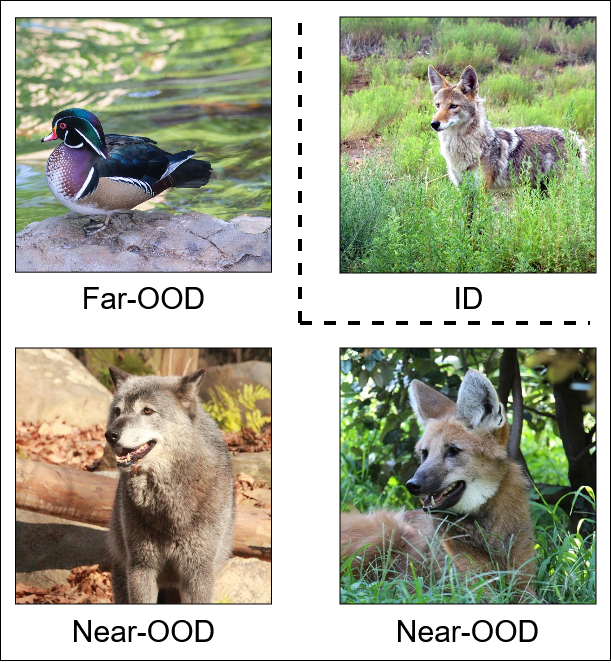
\includegraphics[width=0.9\linewidth]{figures/nearood_example}

  \caption{Detecting OOD samples that are similar to ID samples is a major challenge for OOD detection methods. Considering the coyote in the upper-right corner as the seen (ID) data during training, the bird in the upper-left corner is easy to detect as many features are significantly different (far-OOD). However, the wolf and other coyote sub-species are difficult to detect because they share many similar or overlapping features with the ID data (near-OOD).
  }
  \label{fig:intro-nearood}
\end{figure}

%Despite the importance of OoD detection, existing state-of-the-art methods underperform because they do not sufficiently learn representative information characteristic of ID data. This proposal introduces a novel method that seeks to address this issue and improve OoD detection performance by exploring the use of \textit{multiple views} of data to learn better characteristic ID information. Existing state-of-the-art OoD detection methods and their associated issues are detailed in Section \ref{sec:intro-relwork}. The research thesis, proposed method, and supporting evidence for its contribution are further presented in Section \ref{sec:propwork}. Additional directions for research involving multiple views and OoD detection are suggested in Section \ref{sec:future_work}.
%Although existing OOD detection methods have achieved good performance, they still struggle to detect near-OOD instances \citep{yang2022openood}%, winkens2020contrastive} 

%A significant challenge remaining for OOD detection is the detection of \emph{near-OOD} samples \cite{yang2022openood,winkens2020contrastive}. Near-OOD samples are generally defined as data samples that contain many features that are similar to (or perhaps even overlap) those of ID samples \cite{winkens2020contrastive}. Note that far-OOD samples are simply considered to be data samples with features that are significantly different from ID data features. Intuitively, near-OOD samples are difficult for discriminative classifiers to detect, as such models are designed to extract discriminative features from $\mathcal{D}_{id}$ and similar features in near-OOD data samples deceive the model. Thus, the problem is that existing OOD detection models do not learn \emph{discriminative features} that are sufficiently and distinctly representative of ID class objects. Instead, the deceptive features, henceforth referred to as \emph{spurious features} \cite{neuhaus2023spurious}, are included during learning. Spurious features are not guaranteed to be from the ID distribution and mislead models at test-time when OOD samples may be encountered \cite{ming2022impact,paullada2021data}. This problem is diminished in traditional classification learning as the \emph{i.i.d.} assumption assures that the identical training and test data distributions allow for both discriminative and spurious features to correlate with classes. In OOD detection, this guarantee does not exist, as the OOD (i.e. testing) data distribution is different from that of the ID (i.e. training) distribution $\mathcal{P}_{id}$. Learning class-relevant ID discriminative features is critical because they establish boundaries between ID classes and OOD instances in the feature space, enabling more accurate identification of ID target objects (and subsequently OOD data samples).
Despite the importance of \gls{ood} detection in developing ML systems for open-world settings, significant challenges remain. In particular, the ambiguity between \gls{id} data distributions and all possible \gls{ood} data in the \gls{ood} data distribution allows for extremely difficult cases where \gls{ood} data is similar to samples from the \gls{id} data distribution seen by the model. Consider the above example of the coyote and wolf in the nature preserve \gls{ood} detection application. During training, the ML model saw images of coyotes and learned feature information on coyotes in the \gls{id} data distribution. However, when a wolf appeared during testing, many features from the wolf were similar to or overlapped with those from the coyotes. Given the ML model had only seen animals like coyotes in the \gls{id} data, it would struggle to identify the wolf as an \gls{ood} data sample. This problem is exacerbated if different sub-species of coyotes are considered. If one sub-species of coyote is included in the \gls{id} data distribution and a different sub-species of coyote is encountered during test time, the ML model would have significant difficulty in detecting the different coyote species as \gls{ood}. \ref{fig:intro-nearood} illustrates this example. Here is another example from the text data domain. Imagine an ML model is trained to handle user queries on banking topics related to renewal of a card. The \gls{id} data contains many queries related to card renewal, such as \texttt{Why isn't my card available for use anymore? Did it expire?}, but the model encounters various \gls{ood} queries during testing. Some \gls{ood} queries may be clearly \gls{ood}, for example if the query is asking the model about a loan, e.g. \texttt{I'd like to be considered for a loan, what should I do?}. However, other \gls{ood} queries may be deceptively similar to the \gls{id} data distribution, closely aligning with the ``card renewal'' \gls{id} data. If an \gls{ood} query was asking the model about card cancellation, perhaps with \texttt{My card is close to expiring, can you make my card unavailable for further use?}, the ML model may have a hard time identifying the sample as \gls{ood} given its similarity to \gls{id} data it has seen.

These examples illustrate the challenge of \textbf{near-\gls{ood}} detection \cite{yang2022openood,winkens2020contrastive}. The definition of near-\gls{ood} samples encapsulates the above provided examples. \gls{ood} data that contain features similar to (including overlapping with) those in the \gls{id} data distribution are ``near-\gls{ood}'' \cite{winkens2020contrastive}. This also establishes the definition of \textit{far-\gls{ood}} samples, which are \gls{ood} data that are clearly different from data in the \gls{id} data distribution. Intuitively, near-\gls{ood} data is significantly more difficult for discriminative classifier ML models to detect, as such models are designed to extract and learn features from the \gls{id} data distribution \cite{rubinstein1997discriminative,liu2012discriminative}. As near-\gls{ood} data by definition contains features similar to \gls{id} data, they deceive the model and are harder to detect by nature of lying close to the discriminative decision boundaries learned by such models and methods. The source of the challenge for near-\gls{ood} data is thus in the limited ability of ML models to learn \textit{discriminative features} that sufficiently and distinctly represent the \gls{id} classes (which are an approximate simplification of the \gls{id} data distribution commonly used across the space of ML classification and \gls{ood} detection \cite{kim2015deep,wang2016machine,hendrycks2017baseline}). Instead, deceptive features, denoted as \textit{spurious features} \cite{neuhaus2023spurious}, are learned from the \gls{id} data. Spurious features are not guaranteed to exclusively belong to the \gls{id} data distribution, and learning of such features can mislead ML models during testing when near-\gls{ood} samples may be encountered \cite{ming2022impact,paullada2021data}.

Importantly, this problem is diminished in traditional classification task environments (including those under the \textit{closed-world} assumption) as the \textit{i.i.d.} assumption assures that the training and testing data distributions are identical. This allows for both discriminative and spurious features to correlate with data (and classes) across distributions, providing benefits for the model with no risk of misleading. However, in \gls{ood} detection, this assumption does not apply and thus the guarantee does not exist. The distribution of \gls{ood} data is not the same as the \gls{id} distribution. Spurious features can be present in the \gls{id} testing data \textit{and} the \gls{ood} testing data, which misleads the ML model into recognizing near-\gls{ood} samples with overlapping spurious features instead of detecting them as \gls{ood}. The solution is for ML models to learn \textit{\gls{id} class-relevant discriminative features} because they define distinctive boundaries in the embedding space between \gls{id} classes and \gls{ood} samples. This enables improved detection of \gls{ood} samples with respect to the learned \gls{id} classes and data distribution.

% - (sec) solution directions for image and text, requiring accessible/efficient AND effective
%  + issue is not just achieving good performance with near-OOD, need to also focus on designing solutions that are feasible for application
%  + this implies not only efficacy but efficiency and accessibility
%  + leveraging existing data, solutions, and models boosts accessibility
%  + tuning and pre-training/testing-only methods boost efficiency
%  + prompt-only boosts accessibility
\section{Real-World Solution Directions for Near-OOD Detection}

Solving the near-\gls{ood} detection problem in the context of the open-world setting not only requires the targeted leveraging of \gls{id} class-relevant discriminative features but also requires consideration of applying near-\gls{ood} detection-capable ML systems in real-world environments. From the perspective of a user, it is not only \textit{effectiveness} that is necessary but also \textit{efficiency} and \textit{accessibility} \cite{yuhas2021embedded,li2025secure,wang2025enabling}. Efficiency embodies the optimization of cost for a solution, encapsulating resource requirements with respect to time (data) space. Accessibility embodies the ease-of-use for any given application-side entity (be it developer or end-user). An \gls{ood} detection solution that is highly effective but is intractably expensive in time and computing resources is impossible to develop for and produce in a real setting. Likewise, a solution that requires significant user effort limits its applicability and indirectly reduces overall effectiveness.

\begin{figure}[t]
 \centering
 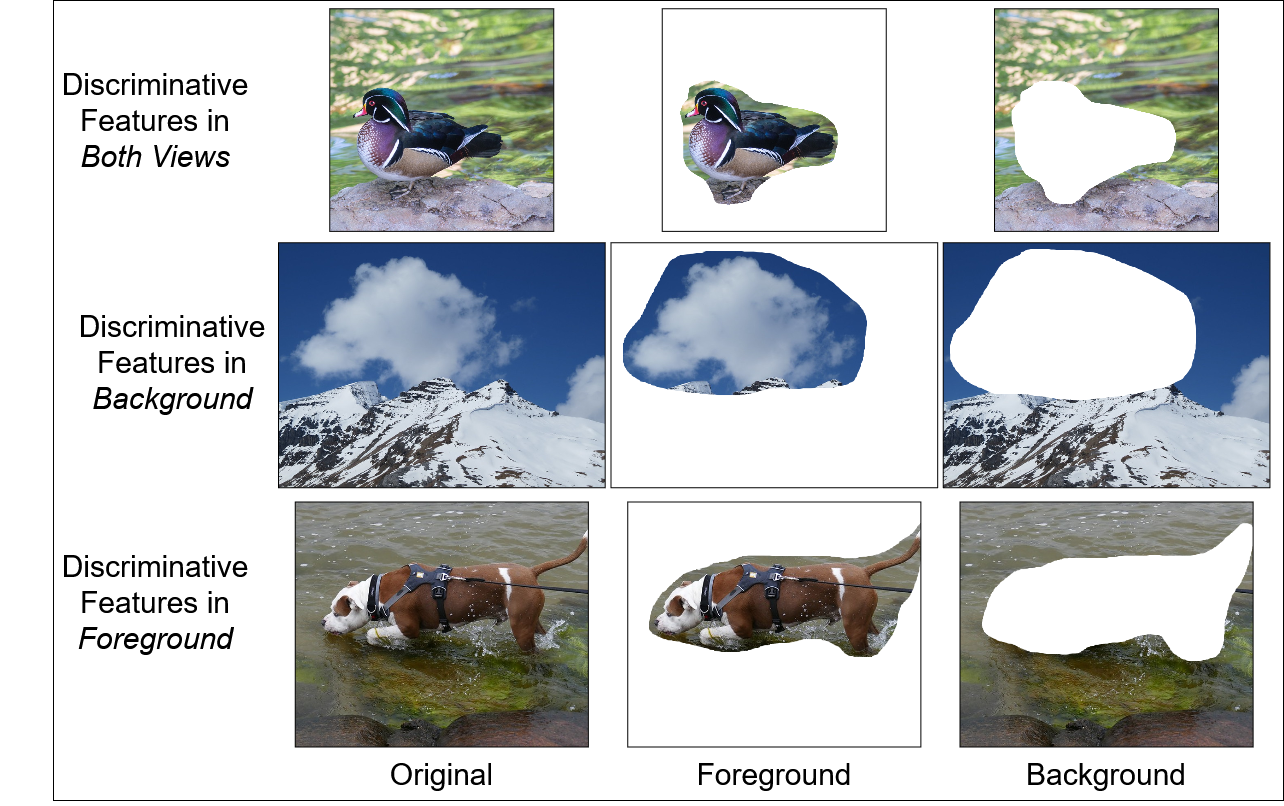
\includegraphics[width=0.95\linewidth]{figures/casod_mv_example}
  \caption{
  %\textcolor{red}{TODO: update} 
  %Foreground and background views contain different ID class-relevant discriminative features for class identification. 
  ID class-relevant discriminative features may appear in any (original, foreground, or background) view of an image, or even in multiple views. Leveraging of these features for OOD detection requires cross-view modeling. Graphic from \cite{politowicz2025casod}. %Segmented views can help models learn important view-specific features and fuse them appropriately.
  }
  \label{fig:intro-mvexample}
  %\vspace{-0.1cm}
\end{figure}

%~(see Sec. \ref{sec:results}). A primary reason is that they do not learn discriminative features that are characteristic of the main object in ID classes well because they consider an \textit{image as a whole}, including both class-relevant and class-irrelevant regions. This often makes them learn spurious or short-cut features \citep{neuhaus2023spurious}, misleading the OOD detection \citep{ming2022exploit}. Using \textbf{only} a \textit{single view} (i.e. the original input image) is thus often \textbf{not enough} for the learner to learn ID class-discriminative features effectively, especially considering challenging near-OOD instances. Extracting and leveraging multiple views (each providing different but complementary information) of the same image can help the learner to better recognize distinguishing characteristics of target object(s) and their relations with the context. Biological systems also support this notion -- it is hypothesized that humans use multiple views to identify what is being observed \citep{weiner2016anatomical}. 

%  + leveraging existing data, solutions, and models boosts accessibility
%  + tuning and pre-training/testing-only methods boost efficiency
%This paper proposes to segment each image into its \textit{foreground} and \textit{background} views and combine them with the original image for OOD detection\footnote{While other options for views, e.g.  crop, rotation \& noise, or image augmentation exist, we noted that the presence of discriminative feature and object's context can be well captured using foreground and background views, which in turn improves OOD detection effectively (see Sec. \ref{sec:disc-ablation}).}. Figure \ref{fig:onecol_vfp} shows examples of three original images and their corresponding foreground and background views. We observe that either the foreground or the background and sometimes both (as in the original image) can contain critical ID class-discriminative features \cite{xiaonoise}. %zhu2017object,xiaonoise}. 
%For example, in Figure \ref{fig:onecol_vfp}, the \textit{Dog}-class image discriminative (object) features are primarily in the foreground while the \textit{Mountain}-class features are primarily in the background. The \textit{Duck}-class image features are in both, with the background water and foliage containing well-separated semantic context in the original view. Thus, depending on the class, all three views becomes important and can contribute in different proportions in the overall learning of the ID class-discriminative features. It is important to note that, although the original image (i.e., original view) contains all information present in the foreground and background views, it often becomes hard for learners to \textit{automatically isolate these views} (and the discriminative information they contain) during feature learning in a \textit{single-view learning framework}. Thus, by segmenting the image into three views (i.e., \textit{original}, \textit{foreground} and \textit{background}), we encourage the learner to explicitly consider useful information from different views and fuse them effectively, resulting in better discriminative feature representation for OOD detection.

%Overall, this isolation of class-relevant discriminative features facilitates learning of only discriminative features informative on ID class objects while simultaneously separating spurious features that otherwise mislead models. Observations in biological systems support the viability of this notion: it has been hypothesized that humans use multiple views of objects, scenes, etc. to perform rapid visual identification \cite{weiner2016anatomical,vuilleumier2002multiple}. Furthermore, foreground-background views are actively considered in biological systems \cite{vuilleumier2002multiple,weiner2016anatomical}, in image processing literature \cite{lin2021real}, and in industry (e.g. autonomous driving) \cite{drygala2022background}, making this approach relevant for modern applications and technology. Despite this, there has been little investigation into the intersection of multi-view data and OOD detection.
When considering the image data domain, a major obstacle to realistic near-\gls{ood} detection is the requirement of significant computational processing. Training expensive image-processing ML models demands significant resources and time-consuming curation of additional data \cite{houlsby2019parameter,hu2021lora,ridnik2021imagenet}. However, these demands can be mitigated through the use of existing resources that also provide additional information beneficial to \gls{ood} detection. For example, existing research in biological systems suggests that humans use multiple views, or alternative augmentations of an image, to identify what is being observed \cite{weiner2016anatomical,vuilleumier2002multiple}. Extracting and leveraging multiple views of an image, each containing different complementary information, could help ML models learn to better recognize distinguishing features of \gls{id} data via the contextual relationships across views. Take \ref{fig:intro-mvexample} as an example. Three original images and their corresponding foreground and background views are depicted, each on their own row. The \textit{Dog}-class image's discriminative features (i.e. those representing the object of ``Dog'') are primarily in the foreground and the separate views isolate these features from the background. The \textit{Mountain}-class image's discriminative features are primarily in the background and the separate views instead isolate these features from the foreground. In both cases, the corresponding view with discriminative features provides additional context that correlates with the original image, reinforcing the features to learn for the \gls{id} data distribution and removing spurious features. This benefit is not isolated to exclusive foreground or background cases. The \textit{Duck}-class image's discriminative features are in both views, with the water and foliage in the background containing informative semantic context that well-separates the class in the \gls{id} data space. Depending on the class, all three views may be important and can contribute to learning of \gls{id} class-relevant discriminative features in different proportions. This provides intuitive benefits over otherwise-equivalent single-view methods (i.e. which only use the original image) which \textit{must} include spurious features with discriminative features in the input, increasing the load on the model during learning to separate the discriminative features in addition to learning them. The \textit{existence of segmented datasets}, including \textit{efficient segmentation models}, establishes a justification for the considered novel \gls{ood} detection approach leveraging multiple foreground and background views by eliminating additional work in procuring such data \cite{lin2021real,drygala2022background,jocher2020ultralytics,qin2020u2}. Further efficiency and accessibility can be embodied by using existing \textit{pre-trained models} and \textit{parameter-efficient fine-tuning} to avoid expensive training costs with impractically high resource demands \cite{hu2021lora,sun2022out,chen2021empirical}. This motivates the development of \gls{sys} \cite{politowicz2026improving}, presented in detail in Chapter \ref{diss_casod} with additional supporting material preceding it in Chapter \ref{diss_mvood_init}.

%\textcolor{blue}{An example of how this isolation benefits OOD detection is presented in TODO( - figure). For the ID sample (left column), the original and foreground views contain the class-relevant ID discriminative features, demonstrated by the recognition of the ID target object and accurate classification. For the simple far-OOD  sample (middle column), all views are very different from the ID sample, with little presence of spurious features. However, for the hard near-OOD samlpe (right column), the features in the original and foreground views are \emph{spurious}, i.e. similar to those of the ID sample. This misleads both views to give high confidence (low OOD scores) to the OOD sample. Only the background view contains features that are significantly different from the ID sample features, resulting in low confidence (high OOD score) and successful detection of the OOD sample.} 

%  + leveraging existing data, solutions, and models boosts accessibility
%  + prompt-only boosts accessibility
For the text data domain, a similar obstacle and solution approach exists. With the advent of large language models (LLMs), application of ML systems is accelerating with increasing demands for more powerful and effective models \cite{angrisani2026gaps,minaee2024large}. However, training such LLMs requires an astronomical amount of computing resources, data, and power. There are consequences for these demands that inspire approaches avoiding the need for training \cite{ding2024sustainable}. Instead, with the known abilities of LLMs to embody and utilize learned pre-trained knowledge \cite{kumar2025llm}, it would be ideal if the benefits of near-\gls{ood} detection could be realized using \textit{only the LLM itself}. That is, implementing effective near-\gls{ood} detection without requiring any sort of interfacing with the LLM's components or underlying outputs (i.e. non-text generation outputs). This inspires the idea of using only \textit{prompts} to induce reasoning in the LLM leading to principled detection of a test input as \gls{id} or \gls{ood}. With the extensive knowledge embedded in LLMs from pre-training, extraction of the discriminative features in the test input relative to the discriminative features of the \gls{id} data distribution is feasible \cite{kumar2025llm,wang2024beyond}. Comparison of the resultant sets of discriminative features through alignment of the various similarity spaces defined by these features, e.g. lexical (comparing words and phrases) and semantic (comparing meanings), informs the weighting of the test input between \gls{id} and \gls{ood}. By limiting the solution to only a prompt, an LLM's basic interface, and the LLM's response, near-universal accessibility is guaranteed, requiring only access to an LLM and some data. This further guarantees efficiency as no training is required. This motivates the development of \gls{syst} \cite{politowicz2026achieving}, presented in detail in Chapter \ref{diss_atpo}.

% - thesis statement: OOD detect, particularly near-OOD detect, is improved in the image domain via fg-bg segmented images in multi-view CVCA and in the text domain via prompt-only, embodying not only performance effectiveness but also efficiency and accessibility

%The primary argument in this proposal is that the use of a single view (i.e. the input image data sample) is not optimal for the learning of discriminative features. Note that for the rest of this proposal, only the domain of image data is considered. Spurious features are included in the sample and interfere with the class-relevant discriminative semantic features necessary for OOD detection. Instead, explicitly separating foreground discriminative features and background features allows for OOD detection models to learn from data with isolated class-relevant information in images. 
%The problem of Out-of-Distribution (OOD) detection has been thoroughly researched but continues to underperform in "near-OOD" settings, where OOD data may be very similar or inseparable from in-distribution (ID) data. The problem is that current state-of-the-art OOD detection methods fail to learn and utilize ID class-representative discriminative features effectively, while simultaneously demanding inaccessible amounts of resources. This thesis presents two OOD detection methods that exhibit state-of-the-art performance in near-OOD settings, one in the image data domain via the use of multi-view cross-attention processing of segmented images, and one in the text data domain using efficient and accessible prompt-only detection via alignment and scoring. The first approach leverages the segmented data and segmentation models to employ a multi-view method for image-based OOD detection, denoted as Cross-view Attention of Segmented views for OOD Detection (CASOD). Through the use of a pre-trained model and a novel cross-view correlation attention fusion architecture, discriminative features are learned across the original image and a foreground and background view, resulting in a highly informative ID class-relevant feature space. Utilizing distance-based OOD detection methods, CASOD achieves state-of-the-art performance over previous OOD detection baselines across a number of academically- or publicly-available datasets, including ImageNet, NINCO, SSB-Hard, iNaturalist, Textures, OpenImage-O, Places365, Species, and SUN. In particular, OOD detection performance on near-OOD datasets is shown to significantly improve. The second approach utilizes the inherent knowledge and reasoning capabilities in large language models (LLMs) to solve the task of prompt-only OOD detection, which requires only the use of text-prompting for OOD detection with no access to LLM components, logits, or outputs and no fine-tuning. Through prompting LLMs to perform lexical and semantic alignment before giving an OOD score for the input, OOD detection on academically- or publicly-available near-OOD datasets, including the Banking, CLINC, StackOverflow, 20NewsGroups, Dbpedia, and Snips datasets, can be significantly improved. Experiments demonstrate that this method, denoted as Alignment-based Thresholding for Prompt-only OOD detection (ATPO), not only outperforms the previous prompt-only OOD detection method but also outperforms strong traditional OOD detection methods with access to LLM features and logits.
\textit{\underline{Thesis Statement:}}
This thesis demonstrates the state-of-the-art effectiveness of two OOD detection methods that were proven against near-OOD datasets in experiments against recent, competitive baselines while additionally fulfilling efficiency and accessibility requirements for real-world application. The first method focuses on the image data domain and utilizes multi-view processing of segmented foreground and background views to learn ID class-relevant discriminative features via a novel cross-view correlation attention feature fusion architecture. Usage of a pre-trained model with parameter-efficient fine-tuning, on top of a fast segmentation model, maintains low computational complexity and simple interfacing between image data and segmented views. Efficient leveraging of segmented foreground and background views results in improved near-OOD detection performance in challenging experimental settings. The second method investigates OOD detection in the text data domain through the use of only text prompts with no complex model components, ML programming expertise, data curation, or model training. Through the induction of lexical and semantic alignment-based reasoning in LLMs, effective near-OOD detection across a variety of settings can be achieved through the processing of scores informed by the ID data. By requiring only a prompt and an LLM with no training, any sort of user barrier is removed ensuring accessibility and efficiency.